\documentclass[18pt]{beamer}

\usetheme{metropolis}
\usefonttheme{professionalfonts}


%% "Patch" to keep the text widths' of Metropolis similar to that of Madrid.
%\setbeamersize{text margin left=15pt, text margin right=15pt}
%\makeatletter
%\setbeamertemplate{title page}{
%\centering
%  \begin{minipage}[b][\paperheight]{.9\textwidth}
%    \ifx\inserttitlegraphic\@empty\else\usebeamertemplate*{title graphic}\fi
%    \vfill%
%    \ifx\inserttitle\@empty\else\usebeamertemplate*{title}\fi
%    \ifx\insertsubtitle\@empty\else\usebeamertemplate*{subtitle}\fi
%    \usebeamertemplate*{title separator}
%    \ifx\beamer@shortauthor\@empty\else\usebeamertemplate*{author}\fi
%    \ifx\insertdate\@empty\else\usebeamertemplate*{date}\fi
%    \ifx\insertinstitute\@empty\else\usebeamertemplate*{institute}\fi
%    \vfill
%    \vspace*{1mm}
%  \end{minipage}
%}
%\makeatother

% Modify the text widths' of section title pages. See `beamerinnerthememetropolis.dtx`.
% `\paperheight` requires adjustment after modifying the frame content placement. Not sure why.
\makeatletter
\setbeamertemplate{section page}{
  \centering
  \begin{minipage}[c][.95\paperheight]{.9\textwidth}
    \raggedright
    \usebeamercolor[fg]{section title}
    \usebeamerfont{section title}
    \insertsectionhead\\[-1ex]
    \usebeamertemplate*{progress bar in section page}
    \par
    \ifx\insertsubsectionhead\@empty\else%
      \usebeamercolor[fg]{subsection title}%
      \usebeamerfont{subsection title}%
      \insertsubsectionhead
    \fi
  \end{minipage}
  \par
  \vspace{\baselineskip}
}
\makeatother

% Make frametitles larger and place closer to center. See `beamerinnerthememetropolis.dtx`.
\setbeamerfont{frametitle}{size=\Large}
\makeatletter
% Theme default adds paddings of 2.2ex to all the four sides of frame titles
\newlength{\metropolis@frametitle@toppadding}
\newlength{\metropolis@frametitle@bottompadding}
\setlength{\metropolis@frametitle@toppadding}{3.5ex} 
\setlength{\metropolis@frametitle@bottompadding}{0ex} 
\setlength{\metropolis@frametitle@padding}{4ex} % Horizontal padding to left
\renewcommand{\metropolis@frametitlestrut@start}{
  \rule{0pt}{\metropolis@frametitle@toppadding +%
    \totalheightof{%
      \ifcsdef{metropolis@frametitleformat}{\metropolis@frametitleformat X}{X}%
    }%
  }%
}
\newcommand*\getlength[1]{\number#1}
\renewcommand{\metropolis@frametitlestrut@end}{%
  \ifnum\getlength{\metropolis@frametitle@bottompadding}>0%
    \rule[-\metropolis@frametitle@bottompadding]{0pt}{\metropolis@frametitle@bottompadding}%
  \fi%
}
\makeatother

% Move up the frame content a bit. See:
% https://github.com/matze/mtheme/blob/master/source/beamerinnerthememetropolis.dtx#L509-L523
% https://tex.stackexchange.com/questions/247826/beamer-full-vertical-centering
\makeatletter
\define@key{beamerframe}{c}[true]{% centered
  \beamer@frametopskip=0pt plus 0.5fill\relax% Default is `1fill`
  \beamer@framebottomskip=0pt plus 1.5fill\relax%
  \beamer@frametopskipautobreak=0pt plus .4\paperheight\relax%
  \beamer@framebottomskipautobreak=0pt plus .6\paperheight\relax%
  \def\beamer@initfirstlineunskip{}%
}
\makeatother


%% Packages
\usepackage[english]{babel}
\usepackage{graphicx}
\usepackage{mathtools} % For \coloneqq (among others)
\usepackage{subcaption}
\usepackage{bm}
\usepackage{dsfont}
\usepackage{soul}
\usepackage{tikz}
\usepackage{pgfplots}
\usetikzlibrary{bayesnet}
%\usepackage[normalem]{ulem}
%	\renewcommand{\ULthickness}{.6pt} % default is 0.4pt
%	\newcommand{\coloredUline}{\bgroup\markoverwith{\textcolor{lava}{\rule[-0.5ex]{2pt}{0.6pt}}}\ULon}
\usepackage{natbib}
	\bibliographystyle{abbrvnat}
	\setcitestyle{authoryear, open={(}, close={)}}
\usepackage{usebib}
\usepackage{bibentry} % For \nobibliography
\newbibfield{journal}
\bibinput{references}


%% Beamer options.
\setbeamercovered{dynamic}
\setbeamercovered{invisible}
\beamertemplatenavigationsymbolsempty
%\setbeamertemplate{caption}{unnumbered}
\setbeamertemplate{footline}{}
%\setbeameroption{show notes on second screen}

%% Customize styles inside itemize environments
%\settowidth{\leftmargini}{\usebeamertemplate{itemize item}}
%\addtolength{\leftmargini}{-1.2\labelsep}
\setbeamerfont{itemize/enumerate subbody}{size=\normalsize} %to set the body size
\setbeamertemplate{itemize subitem}{\normalsize\raise1.25pt\hbox{\donotcoloroutermaths$\blacktriangleright$}}  % to set the symbol size

%% Custom environments
\newcommand{\defineTightSpacing}{%
	\setlength{\abovedisplayskip}{.25\baselineskip}%
	\setlength{\belowdisplayskip}{.25\baselineskip}%
}
\newcommand{\reduceLeftmargin}[1][1]{%
	\addtolength{\leftmargini}{-#1\labelsep}%
	\addtolength{\leftmarginii}{-#1\labelsep}%
}
\newenvironment{tightEquation}{%
	\defineTightSpacing%
	\begin{equation}
}{
	\end{equation} \ignorespacesafterend
}
\makeatletter
\newenvironment{tightEquation*}{%
	\defineTightSpacing%
	\begin{equation*}
}{
	\end{equation*} \ignorespacesafterend
}
\newcommand{\defineWithinItemizeSpacing}{%
	\setlength{\abovedisplayskip}{.3\baselineskip}%
	\setlength{\belowdisplayskip}{.3\baselineskip}%
}
\newenvironment{itemizedEquation}{%
	\defineWithinItemizeSpacing%
	\begin{equation}
}{
	\end{equation} \ignorespacesafterend
}
\makeatletter
\newenvironment{itemizedEquation*}{%
	\defineWithinItemizeSpacing%
	\begin{equation*}
}{
	\end{equation*} \ignorespacesafterend
}
\newenvironment{indented}[1][3]{%
	\hfill \begin{minipage}{\dimexpr\textwidth-#1ex} 
	}{
	\end{minipage}
}
\newenvironment{wideitemize}{%
  \begin{itemize}
  \addtolength\itemsep{.4\baselineskip}
}{
  \end{itemize}
}
\newenvironment{tightItemize}[1][]{%
  \vspace{-.3\baselineskip}%
  \begin{itemize}[#1]
  \addtolength\itemsep{-.1\baselineskip}
}{
  \end{itemize}
}
\newenvironment{tightEnumerate}[1][1.]{%
  \vspace{-.3\baselineskip}%
  \begin{enumerate}[#1]
  \addtolength\itemsep{-.1\baselineskip}
}{
  \end{enumerate}
}

%% Color definitions
\definecolor{turquoise}{rgb}{0.19, 0.84, 0.78}
\definecolor{mediumturquoise}{rgb}{0.28, 0.82, 0.8}
\definecolor{lava}{rgb}{0.81, 0.06, 0.13}
\colorlet{linkColor}{mediumturquoise}
\colorlet{highlightedTextColor}{lava}

%% Set the color theme of the presentation
\definecolor{jhuBlue}{RGB}{0, 45, 114} % "Heritage" blue; https://brand.jhu.edu/color/
\definecolor{jhuSpiritBlue}{RGB}{114, 172, 229} % lighter blue
\colorlet{themecolor}{jhuBlue}
\colorlet{bgcolor}{themecolor}
\colorlet{textcolor}{white}
\usecolortheme[named=themecolor]{structure}
%\setbeamercolor{titlelike}{fg=black}
\setbeamercolor{frametitle}{fg=themecolor, bg=white}
\setbeamercolor{section in head/foot}{fg=textcolor}
\setbeamercolor{background canvas}{bg=white}
%\colorlet{toccolor}{black}
%\setbeamercolor{section in toc}{fg=toccolor}
\setbeamercolor{block title}{bg=themecolor!75!gray!25}
\setbeamercolor{block body}{bg=themecolor!75!gray!5}


% Macros

%% Utility macros
\newcommand{\noteBullet}{\hspace*{.75em}\textcolor{themecolor}{$\blacktriangleright$}\ }
\renewcommand{\textsc}[1]{{\small \MakeUppercase{#1}}}

%% General math macros
\newcommand{\given}{\mskip.7\thinmuskip | \mskip.7\thinmuskip}
\newcommand{\midGiven}{\mskip.7\thinmuskip \middle| \mskip.7\thinmuskip}
\newcommand{\spacedColon}{\mkern .5mu : \mkern 1mu}
\newcommand{\spacedEq}{\mkern 1mu = \mkern 1.5mu}
\newcommand{\divby}{\thinnerspace /}
\newcommand{\defeq}{\vcentcolon =} % `\coloneqq` and `\vcentcolon` requires the `mathtools` package: https://tex.stackexchange.com/questions/194344/symbol-for-definition
\newcommand{\diff}{\operatorname{\mathrm{d}}\!{}}
\newcommand{\sign}{\mathrm{sign}}
\newcommand{\diag}{\mathrm{diag}}
\newcommand{\medcap}{\mathbin{\mathsmaller{\bigcap}}}
\DeclareMathOperator*{\argmin}{argmin}
\DeclareMathOperator*{\argmax}{argmax}
\newcommand{\elemwiseProd}{\odot}
\renewcommand{\complement}{{\raisebox{1.5pt}{\scriptsize $\mathsf{c}$}}}
\newcommand{\transpose}{\text{\raisebox{.5ex}{$\intercal$}}}
\newcommand{\higherTranspose}{\text{\raisebox{.9ex}{$\intercal$}}}
\newcommand{\lowerscript}[1]{\raisebox{-2pt}{\scriptsize $#1$}}
\newcommand{\yesnumber}{\addtocounter{equation}{1}\tag{\theequation}}
\newcommand{\thinnerspace}{\mskip.5\thinmuskip}
\newcommand{\thinnestspace}{\mskip.25\thinmuskip}
\newcommand{\negthinnerspace}{\mskip-.5\thinmuskip}
\newcommand{\spaceBeforePartial}{\mskip\thinmuskip}
\newcommand{\scriptsumi}{{\scriptsize \sum_i}} % Suscript needs to be within bracket, hence the hard coding
\newcommand{\approxpropto}{%
	\mathrel{\vcenter{
		\offinterlineskip\halign{
			\hfil$##$\cr \propto\cr\noalign{\kern2pt}\sim\cr\noalign{\kern-2pt}
		}
	}}
}
%% Probability / statistics macros
\DeclareMathOperator{\probability}{\mathbb{P}}
\newcommand{\expectation}{\mathbb{E}}
\newcommand{\variance}{\mathrm{Var}}
\DeclareMathOperator*{\covariance}{Cov}
\newcommand{\indicator}{\operatorname{\mathds{1}}}
\newcommand{\eqDistribution}{\mathrel{\raisebox{-.2ex}{$\overset{\scalebox{.6}{$\, d$}}{=}$}}}
\newcommand{\iidSim}{\mathrel{\raisebox{-.3ex}{$\overset{\text{i.i.d.}}{\sim}$}}}
\newcommand{\unifDist}{\mathrm{Unif}}
\newcommand{\normalDist}{\operatorname{\mathcal{N}}}
\newcommand{\betaDist}{\mathrm{Beta}}
\newcommand{\gammaDist}{\mathrm{Gamma}}
\newcommand{\mle}[1]{\widehat{#1}_{\textrm{mle}}}
\newcommand{\map}[1]{\widehat{#1}_{\textrm{map}}}
\newcommand{\empiricalVar}{\widehat{\variance}}
\newcommand{\kldivergence}{D_{\mathrm{KL}}}
\newcommand{\truthSub}{\mathrm{tru}}

%% Variable macros / Aliases
\newcommand{\nPred}{p}
\newcommand{\nObs}{n}
\newcommand{\density}{\operatorname{\pi}}
\newcommand{\likelihood}{L}
\newcommand{\infoMat}{\mathcal{I}}
\newcommand{\by}{\bm{y}}
\newcommand{\bx}{\bm{x}}
\newcommand{\bX}{\bm{X}}
\newcommand{\vecRv}{\mathbf{X}}
\newcommand{\bmu}{\bm{\mu}}
\newcommand{\bbeta}{\bm{\beta}}
\newcommand{\btheta}{\bm{\theta}}
\newcommand{\Id}{\bm{I}}
\newcommand{\bPhi}{\bm{\Phi}}
\newcommand{\bSigma}{\bm{\Sigma}}

%% Hypothesis testing/model selection macros
\newcommand{\hypothesis}{H}
\renewcommand{\action}{A}
\newcommand{\model}{\mathcal{M}}
\newcommand{\loss}{\mathcal{L}}
\newcommand{\nullSub}{\mathrm{nul}}
\newcommand{\altSub}{\mathrm{alt}}
\newcommand{\bayesFacAlt}{B_{\mathrm{a} / \mathrm{n}}}
\newcommand{\nonzeroCoefSet}{J}
\newcommand{\inclusionProb}{q}

\title{%
	\centerline{Bayesian hypothesis testing \& model selection}%
}
\author{%
	Aki Nishimura\\
	Department of Biostatistics%
}
%\institute[]{}
\date{}

\titlegraphic{%
	\begin{picture}(0,0)
		% Try coordinate (155, -150) for a one-line title, (165, -160) if two-lines, and (155, -172) if three-lines
		\put(155, -150){\makebox(0,0)[lb]{
\includegraphics[width=.45\textwidth]{jhsph_biostat_logo}}}
	\end{picture}%
}

\begin{document}

\maketitle


\begin{frame}
\frametitle{Testing null vs.\ alternative in Bayes way}
Let's consider the model $y_i \iidSim \normalDist(\mu, \sigma^2)$ and testing
\begin{equation*} \defineTightSpacing%
\hypothesis_\nullSub: \mu = 0 
	\ \text{ vs.\ } \ 
	\hypothesis_\altSub: \mu \neq 0.
\end{equation*}

\pause
A Bayesian way to formulate of the problem is to ask
\begin{equation*} \defineTightSpacing%
\hypothesis_\nullSub: \mu \sim \delta_0(\cdot) 
	\ \text{ vs.\ } \ 
	\hypothesis_\altSub: \mu \sim \density_\altSub(\cdot) 
\end{equation*}
where $\density_\altSub(\cdot)$ can be taken, for example, as $\normalDist(0, \sigma_\altSub^2)$.

\pause
\smallskip
Having to explicitly specify $\density_\altSub(\cdot)$ is somewhat awkward (though maybe only b/c we've been immersed in the freq testing paradigm).

\pause
But also an opportunity to test a more meaningful hypothesis; e.g.\
\begin{equation*} \defineTightSpacing%
\hypothesis_\nullSub: \mu \sim \unifDist([-\epsilon, \epsilon])
	\ \text{ vs.\ } \ 
	\hypothesis_\altSub: \mu \sim \unifDist([-L, -\epsilon] \cup [\epsilon, L]).
\end{equation*}
\end{frame}


\begin{frame}
\frametitle{Testing null vs.\ alternative in Bayes way}
Under Bayes, hypothesis testing is equivalent to model selection and amounts to calculating $\probability(\hypothesis_\nullSub \given \by)$ and $\probability(\hypothesis_\altSub \given \by)$ according to
\begin{equation*} \defineTightSpacing%
\probability(\hypothesis \given \by)
	\propto \likelihood(\by \given \hypothesis) \probability(\hypothesis).
\end{equation*}

\pause
In particular, the posterior odds in favor of $\hypothesis_\altSub$ are given by
\begin{equation*} \defineTightSpacing%
\frac{%
	\probability(\hypothesis_\altSub \given \by)%
}{%
	\probability(\hypothesis_\nullSub \given \by)
}%
	= \frac{%
		\likelihood(\by \given \hypothesis_\altSub)%
	}{%
		\likelihood(\by \given \hypothesis_\nullSub) 
	}%
	\frac{%
		\probability(\hypothesis_\altSub)%
	}{%
		\probability(\hypothesis_\nullSub) 
	}
	\pause
	= \bayesFacAlt \thinnerspace
	\frac{%
		\probability(\hypothesis_\altSub)%
	}{%
		\probability(\hypothesis_\nullSub) 
	},
\end{equation*}
where the \textit{Bayes factor} $\bayesFacAlt$ summarizes the evidence from $\by$.

\pause
\smallskip
The probabilities themselves can be calculated by noting that 
\begin{equation*} \defineTightSpacing%
1 
	= \probability(\hypothesis_\altSub \given \by) + \probability(\hypothesis_\nullSub \given \by)
	= \probability(\hypothesis_\altSub \given \by) \left(
		1 + \frac{%
			\probability(\hypothesis_\nullSub \given \by)%
		}{%
			\probability(\hypothesis_\altSub \given \by) 
		}
	\right).
\end{equation*}
\end{frame}


\begin{frame}
\frametitle{Bayes factor in testing Gaussian mean}
Let's try calculating the Bayes factor under the hypotheses
\begin{equation*} \defineTightSpacing%
\hypothesis_\nullSub: \mu \sim \delta_0(\cdot) 
	\ \text{ vs.\ } \ 
	\hypothesis_\altSub: \mu \sim \normalDist(0, \sigma_\altSub^2).
\end{equation*}

\pause
Can think of it as a caricature of `spike-and-slab' variable selection:
\vspace*{-1.2\baselineskip}%
\begin{figure}
\centering
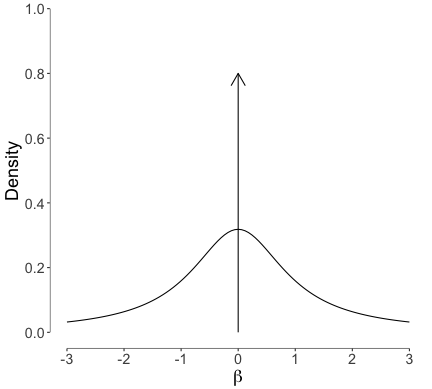
\includegraphics[height=.5\paperheight]{Figure/spike_and_slab}
\end{figure}

\end{frame}

\begin{frame}
\frametitle{Bayes factor in testing Gaussian mean}
Recall that
\begin{equation*} \defineTightSpacing%
\begin{aligned}
\likelihood(\by \given \mu)
	&\propto \frac{1}{\sigma^n}
		\exp\!\left( - \frac{1}{2 \sigma^2} \sum_i (y_i - \bar{y})^2 \right)
		\exp\!\left( - \frac{n}{2 \sigma^2} (\bar{y} - \mu)^2 \right) \\
	&\propto \normalDist\!\left(
		\bar{y} \midGiven \mu, n^{-1} \sigma^2
	\right).
\end{aligned}
\end{equation*}
% Note: We therefore need to only consider the likelihood of the sufficient statistics.

\pause
\smallskip
The (marginal) likelihood under $\hypothesis_\nullSub$ is, therefore, 
\begin{equation*} \defineTightSpacing%
\likelihood(\by \given \hypothesis_\nullSub)
	\propto \normalDist\!\left(
		\bar{y} \midGiven 0, n^{-1} \sigma^2
	\right).
\end{equation*}

\pause
The marginal likelihood under $\hypothesis_\altSub$ is 
\begin{equation*} \defineTightSpacing%
\begin{aligned}
\likelihood(\by \given \hypothesis_\altSub)
	&\propto \int \normalDist\!\left(
		\bar{y} \midGiven \mu, n^{-1} \sigma^2
	\right)
	\normalDist\!\left(
		\mu \midGiven 0, \sigma_\altSub^2
	\right) \diff \mu \\
	&= \normalDist\!\left(
		\bar{y} \midGiven 0, n^{-1} \sigma^2 + \sigma_\altSub^2
	\right).
\end{aligned}
\end{equation*}

\pause
\textbf{Note:} Be careful with constants when computing Bayes factors; 
you can only ignore ones that cancel out when taking the ratio. % $\frac{\likelihood(\by \given \hypothesis_\nullSub)}{\likelihood(\by \given \hypothesis_\altSub)}$.
\end{frame}


\begin{frame}
\frametitle{Bayes factor in testing Gaussian mean}

So the Bayes factor is
\begin{equation*} \defineTightSpacing%
\begin{aligned}
\frac{%
	\likelihood(\by \given \hypothesis_\altSub)%
}{%
	\likelihood(\by \given \hypothesis_\nullSub) 
}
	&= \frac{
		\normalDist\!\left(
			\bar{y} \midGiven 0, n^{-1} \sigma^2 + \sigma_\altSub^2
		\right)
	}{
		\normalDist\!\left(
			\bar{y} \midGiven 0, n^{-1} \sigma^2
		\right)
	} \\
	\pause
	&= \left( 1 + \frac{n \sigma_\altSub^2}{\sigma^2} \right)^{\!-1/2} \!
	\exp\!\left(
		\frac{1}{2} 
		\left[ 1 + \frac{\sigma^2}{n \sigma_\altSub^2} \right]^{-1} \!
		\frac{n \bar{y}^2}{\sigma^2}
	\right).
\end{aligned}
\end{equation*}

\pause
Setting $\bar{z}_n = \frac{\sqrt{n} \thinnerspace \bar{y}}{\sigma} \sim \normalDist\!\left(\! \frac{\sqrt{n} \thinnerspace \mu_\truthSub}{\sigma}, 1 \right)$, we have
\begin{equation*} \defineTightSpacing%
\begin{aligned}
\bayesFacAlt
	&= \left( 1 + \frac{n \sigma_\altSub^2}{\sigma^2} \right)^{\!-1/2} \!
	\exp\!\left(
		\frac{1}{2} 
		\left[ 1 + \frac{\sigma^2}{n \sigma_\altSub^2} \right]^{-1} \!
		\bar{z}_n^2
	\right).
\end{aligned}
\end{equation*}
\end{frame}


\begin{frame}
\frametitle{Asymptotic behavior of Bayes factor}
\pause
To study its behavior as $n \to \infty$, note that
\begin{equation*} \defineTightSpacing%
\begin{aligned}
\bayesFacAlt
	&\sim \frac{1}{\sqrt{n}} 
	\exp\!\left(
		\frac{1}{2} \thinnerspace \bar{z}_n^2
	\right)
	\ \text{ for } \,
	\bar{z}_n \sim \normalDist\!\left(\! \frac{\sqrt{n} \thinnerspace \mu_\truthSub}{\sigma}, 1 \right).
\end{aligned}
\end{equation*}

\pause
\medskip
Under the alternative $\mu_\truthSub \neq 0$, 
$$\displaystyle 
\bayesFacAlt
	\sim \frac{1}{\sqrt{n}} 
	\exp\!\left(
		\frac{1}{2} \thinnerspace \frac{n \mu_\truthSub^2}{\sigma^2}
	\right) \to \infty.$$

\pause
Under the null $\mu_\truthSub = 0$,
$$\displaystyle
\bayesFacAlt \sim \frac{1}{\sqrt{n}} \to 0.$$
\end{frame}


\begin{frame}
\frametitle{Asymptotic behavior of Bayes factor}
This Bayes test is apparently better at accepting the alternative

\pause
--- evidence accumulates much more quickly in favor of the correct hypothesis under the alternative than under the null.

\pause
\smallskip
In fact, this asymptotic behavior of Bayes factor holds more generally under \textit{local} alternatives:
\begin{equation*} \defineTightSpacing%
\hypothesis_\nullSub: \btheta = \btheta_\nullSub
	\ \text{ vs.\ } \ 
\hypothesis_\altSub: \btheta \sim \density_\altSub(\cdot)
	\, \text{ with } \density_\altSub(\btheta_\nullSub) > 0.
\end{equation*}

\pause
Faster evidence accumulation under null can be achieved by using a \textit{non-local} alternative $\density_\altSub(\btheta_\nullSub) = 0$ \citep{johnson2010nonlocal}.
\end{frame}


\begin{frame}
\frametitle{Asymptotic behavior of Bayes factor}
\begin{figure}
\centering
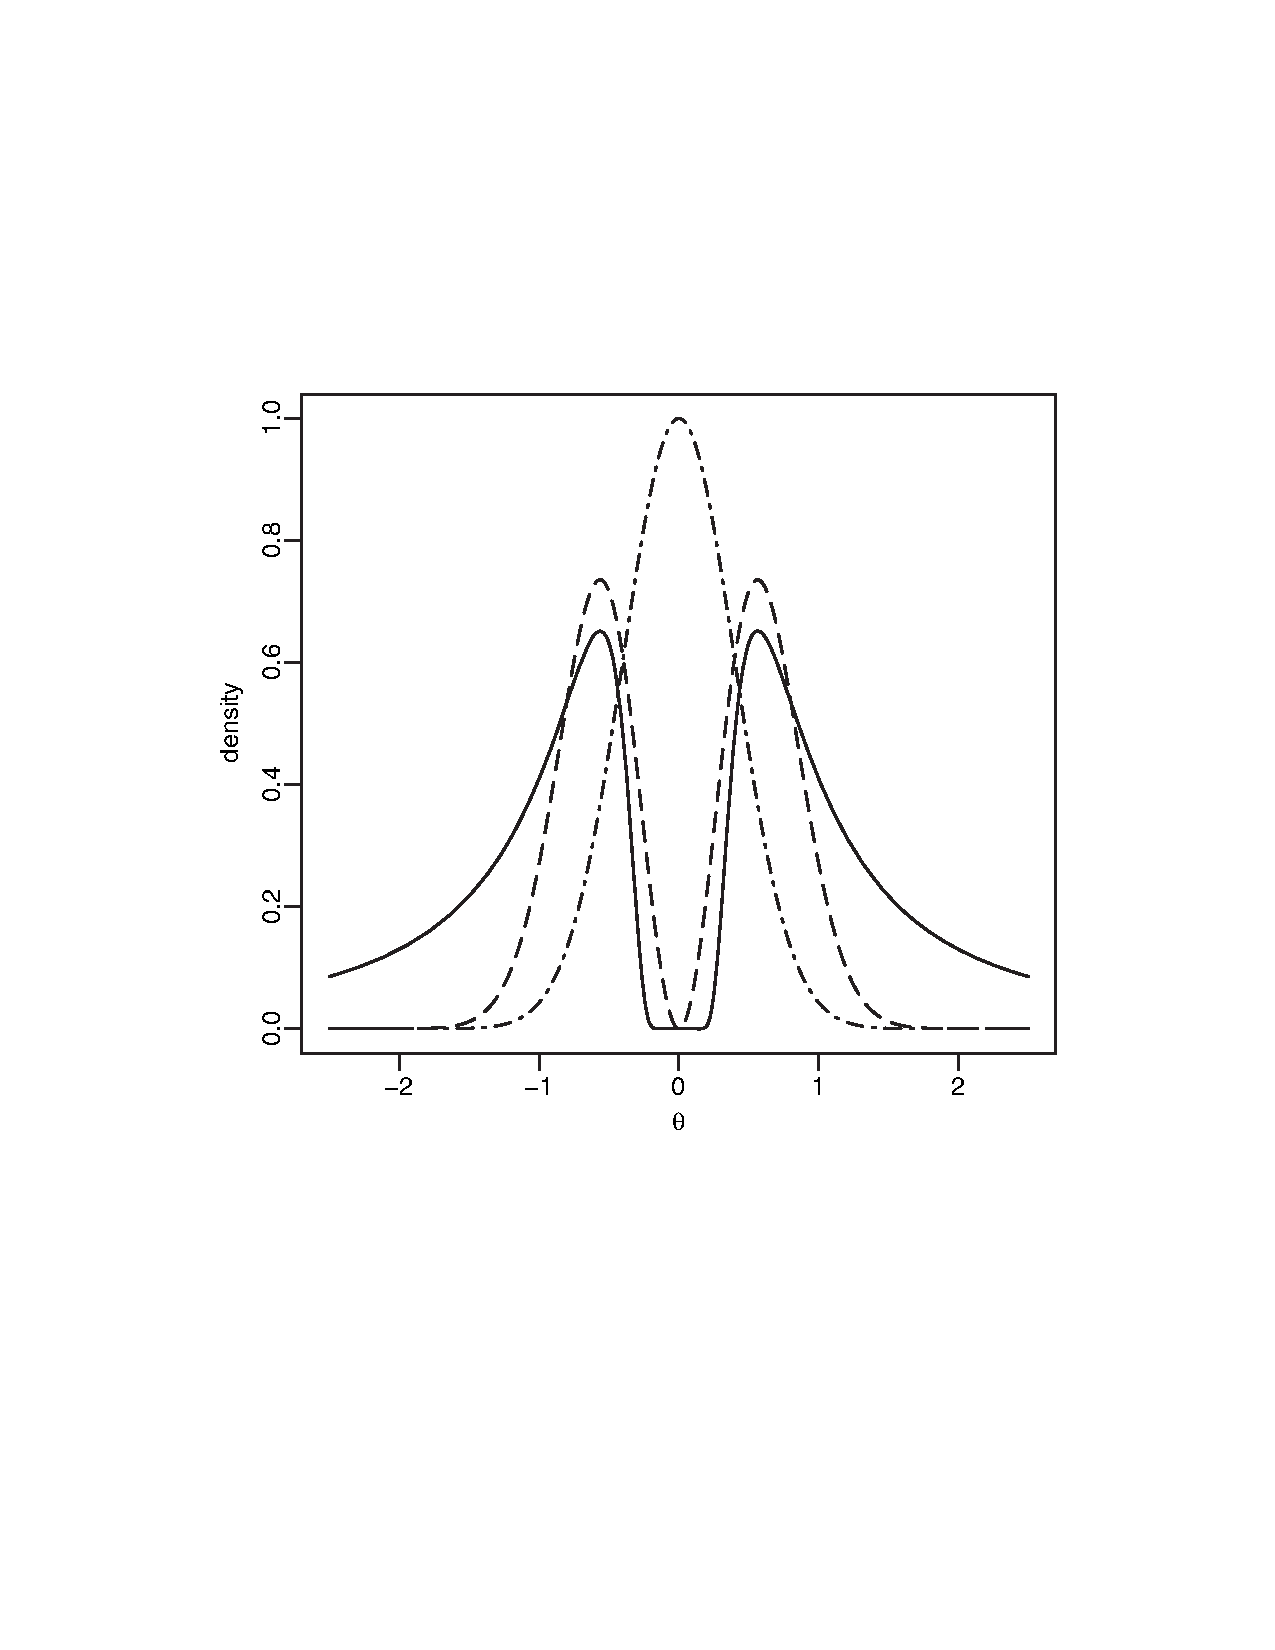
\includegraphics[width=.9\linewidth]{Figure/non_local_prior}
\caption*{\textcolor{themecolor}{\textbf{Figure:}}
	Comparison of the $\thinnerspace \normalDist(0, 1)$ prior with two  non-local priors.
}
\end{figure}
\end{frame}


\begin{frame}
\frametitle{Jeffreys-Lindley ``Paradox''}
Let's now take another, different look at the Bayes factor: 
\begin{equation*} \defineTightSpacing%
\begin{aligned}
\bayesFacAlt
	&= \left( 1 + \frac{n \sigma_\altSub^2}{\sigma^2} \right)^{\!-1/2} \!
	\exp\!\left(
		\frac{1}{2} 
		\left[ 1 + \frac{\sigma^2}{n \sigma_\altSub^2} \right]^{-1} \!
		\bar{z}_n^2
	\right) \\
	&\sim \frac{1}{\sqrt{n}} 
		\exp\!\left(
			\frac{1}{2} \thinnerspace \bar{z}_n^2
		\right)
	\ \text{ for } \
	\bar{z}_n = \frac{\sqrt{n} \thinnerspace \bar{y}}{\sigma}.
\end{aligned}
\end{equation*}

\pause
\smallskip
Let's imagine $\bar{z}_n = 2$, so that a frequentist would reject the null.

\pause
\smallskip
But the $1 / \sqrt{n}$ factor mean $\bayesFacAlt$ could be small, so that a Bayesian would favor the null. (!)

\pause
\smallskip
This potential disagreement is known as (Jeffrey-)Lindley paradox.

\pause
Of course, this isn't a real paradox b/c the two tests are asking two different questions; 
e.g.\ you never ``accept'' the null in a freq test.
\end{frame}


\begin{frame}
\frametitle{Bartlett's ``Paradox''}
Let's take one another look at the Bayes factor: 
\begin{equation*} \defineTightSpacing%
\begin{aligned}
\bayesFacAlt
	&= \left( 1 + \frac{n \sigma_\altSub^2}{\sigma^2} \right)^{\!-1/2} \!
	\exp\!\left(
		\frac{1}{2} 
		\left[ 1 + \frac{\sigma^2}{n \sigma_\altSub^2} \right]^{-1} \!
		\bar{z}_n^2
	\right).
\end{aligned}
\end{equation*}
(This time, we are \textit{not} going to let $n \to \infty$.)

\pause
\smallskip
Imagine that we want to be ``uninformative'' about $\mu$ under $\hypothesis_\altSub$, so we take a large $\sigma_\altSub$.
What would happen in this case?

\pause
\smallskip
As $\sigma_\altSub \to \infty$, we have $\bayesFacAlt \to 0$ and \textit{always} accept the null.

\pause
\smallskip
\cite{bartlett1957paradox} observed phenomenon, but these paradoxes are often collectively called (Jeffrey-)Lindley(-Bartlett) paradox.
\end{frame}


\begin{frame}
\frametitle{Danger of ``uninformative/vague'' priors}
Bartlett's paradox is a manifestation of how an ``uninformative'' prior can be \textit{very} informative in an insidious way.

\pause
\smallskip
%To understand the cause of the paradox, imagine observing a test statistics value $\bar{z}_n = 5$ or, equivalently, $\thinnerspace \bar{y} = \frac{5 \sigma}{\sqrt{n}} \sim \normalDist\!\left( \mu, \frac{\sigma^2}{n} \right)$.
To understand the cause of the paradox, note that observed data is most likely when $\mu = \bar{y}$ and equally (un)likely when $\mu = 0$ or $= 2 \bar{y}$.

\pause
\smallskip
In other words, the prior guess $\mu = 0$ is off by $| \bar{y} |$ from the best guess but any other guess with $\left| \mu - \bar{y} \right| > \left| \bar{y} \right|$ even worse.

\pause
\smallskip
The problem with an uninformative prior arises from the fact that
\begin{equation*} \defineTightSpacing%
\probability_\altSub \!\left( \left| \mu - \bar{y} \right| > \left| \bar{y} \right| \right)
	\to 1 \ \text{ as } \, \sigma_\altSub \to \infty;
\end{equation*}
i.e.\ your prior guess under $\hypothesis_\altSub: \mu \sim \density_\altSub(\cdot)$ is further off than $\hypothesis_\nullSub: \mu = 0$ with nearly 100\% chance.
\end{frame}


\begin{frame}
\frametitle{Danger of ``uninformative/vague'' priors}
\textbf{Q.} But, wait, isn't $\density(\mu) \propto 1$ a proven objective prior? 

\pause
\textbf{A.} Yes for parameter estimation, but not for model selection.

\pause
\smallskip
More generally, it's often a bad idea to place vague priors on hyper- parameters, whose main role is to control the model's complexity; 
\pause
\noteBullet e.g.\ across-group variance parameter in hierarchical models. 

\pause
\smallskip
Improper use of uninformative priors one of the most common, and potentially consequential, mistakes among Bayes amateurs.
\end{frame}


\begin{frame}
\frametitle{Bartlett's ``Paradox'' \& Bayesian Occam's razor}
%{\fontdimen2\font=.6ex 
In a more positive light, Bartlett's paradox reveals the complexity control ``Occam's razor'' mechanism built into Bayesian inference.
%}

\pause
\smallskip
When you introduce additional parameter/flexibility in a Bayesian model, you also pay the price by spreading prior probability into regions of parameter space less compatible with the observed data.

\pause
\smallskip
To put it another way, \textsc{mle} picks the best fitting model from however many options given, but Bayesians have a ``fixed budget.''

\pause
\smallskip
Hyper-parameter/model selection through marginal likelihood auto- matically accounts for this trade-off (e.g.\ in regularized regression).
\end{frame}


\begin{frame}
\frametitle{On use of posterior tail-probability for testing}
Sometimes, people use a tail-probability $\probability( \theta > \theta_0 \given \by )$ for some chosen $\theta_0$ as evidence of ``significant effect.''

\pause
\smallskip
While a reasonable heuristic, the tail-probability doesn't really have any formal Bayesian interpretation as a measure of evidence.

\pause
\smallskip
One exception is the case of one-sided testing, where it admits an interpretation as a $p$-value \citep{casella1987onesided_testing}.

\end{frame}


\begin{frame}
\frametitle{On use of posterior tail-probability for testing}
To illustrate the $p$-value interpretation, we consider a one-sided test
\begin{equation*} \defineTightSpacing%
\hypothesis_\nullSub: \mu \leq \mu_0 
	\ \text{ vs.\ } \ 
	\hypothesis_\altSub: \mu > \mu_0
\end{equation*}
under the model $y_i \iidSim \normalDist(\mu, \sigma^2)$.

\pause
\smallskip
We assume $\probability(\hypothesis_\nullSub) = \probability(\hypothesis_\altSub) = \frac12$ and priors
\begin{equation*} \defineTightSpacing%
\hypothesis_\nullSub: \mu \sim \normalDist(\mu_0, \sigma_0^2) \indicator_{(-\infty, \, \mu_0]}
	\, \text{ vs.\ } \,
	\hypothesis_\altSub: \mu \sim \normalDist(\mu_0, \sigma_0^2) \indicator_{(\mu_0, \, \infty]}.
\end{equation*}

\pause
In a sense, this is just a convoluted way to express the familiar prior
\begin{equation*} \defineTightSpacing%
\density(\mu) 
	= \frac{1}{2} \density(\mu \given \hypothesis_\nullSub) + \frac12 \density(\mu \given \hypothesis_\altSub)
	\sim \normalDist(\mu_0, \sigma_0^2).
\end{equation*}

\pause
Consequently, the test amounts to calculating the probabilities of $\mu \leq \mu_0$ and $\mu > \mu_0 $ under 
$\displaystyle \mu \given \by \sim \normalDist\!\left( \frac{\phi_0 \mu_0 + n \phi \bar{y}}{\phi_0 + \phi}, \frac{1}{\phi_0 + n \phi} \right)$.
\end{frame}


\begin{frame}
\frametitle{On use of posterior tail-probability for testing}
For one-sided testing, therefore, calculation of $\bayesFacAlt$, $\probability(\hypothesis_\nullSub \given \by)$, and $\probability(\hypothesis_\altSub \given \by)$ only involves usual estimation problem quantities.

\pause
In particular, use of a flat prior $\density(\mu) \propto 1$ can be justifies as a limit.

\pause
\smallskip
The flat prior leads to the posterior $\displaystyle \mu \given \by \sim \normalDist\!\left( \bar{y}, \thinnerspace \sigma^2 / n \right)$ and to
\begin{equation*} \defineTightSpacing%
%\begin{aligned}
\probability(\hypothesis_\nullSub \given \by)
	= \probability(\mu \leq \mu_0 \given \by) 
	= \Phi\left( \frac{\mu_0 - \bar{y}}{\sigma / \sqrt{n}} \right) 
	= 1 - \Phi\left( \frac{\bar{y} - \mu_0}{\sigma / \sqrt{n}} \right),
%\end{aligned}
\end{equation*}
where the last quantity is the $p$-value for a freq one-sided test.

\pause
\smallskip
Agreement between tail-probability and $p$-value here simply reflects the freq property of Bayesian CI, rather than inherent relationship.
\end{frame}


\begin{frame}
\frametitle{On use of posterior tail-probability for testing}

Takeaway message is \textit{not} that 
\pause
\begin{tightItemize}
\item ``tail-probability can be interpreted as model probability.''
\pause
\item ``$p$-values has a Bayes interpretation as a measure of evidence'' --- it generally doesn't, though mapping $p$-value to obtain a bound on Bayes factor is a possibility\\
\hfill \citep{benjamin2019use_of_pvalue}.
\end{tightItemize}

\pause
The message is rather that 
\pause
\begin{tightItemize}
\item it takes quite a bit of maneuvers to justify a tail-probability as a formal measure of evidence;
\pause
\item even after all the maneuvers, it offers little beyond a $p$-value;
\end{tightItemize}
\pause
\vspace*{-.2\baselineskip}
so let's not a tail-probability too seriously.

%\begin{indented}[2.3]
%``it takes quite a bit of maneuvers to justify a tail-probability as a formal measure of evidence, so let's not take it too seriously.''
%\end{indented}
%
%\medskip
%Even with such maneuvers, a tail-probability doesn't offer much beyond what a $p$-value and freq one-sided test do.
\end{frame}


\begin{frame}
\frametitle{More general Bayesian tests}
Bayesian tests become a particularly attractive option for more complex tests, e.g.\ when hypotheses are not nested.

\pause
For example, you may want to test three possible scenarios for how ground-level ozone changed over time \citep{kass1995bayes_factor}:

\medskip
\begin{minipage}{.32\linewidth}
	\begin{figure}
		\begin{tikzpicture}
		\begin{axis}[
			width=0.48\paperheight,
			height=0.48\paperheight,
		    axis lines = left,
		    xmin=0,
		    xmax=1,
		    ymin=0,
		    ymax=3,
		    xlabel = {\(t\)},
		    ylabel = {\(\)},
		    ticks = none,
		    legend style={
		    	font=\small, 
		    	draw=none, % Remove legend box
		    	empty legend % Remove line marker
		    }
		]
		%Below the red parabola is defined
		\addplot [
			domain=0.01:0.99,
		    samples=99, 
		    color=jhuSpiritBlue,
		    semithick
		]
		{1.5};
		\addlegendentry{\({\tiny \hypothesis_0}\)}
		\end{axis}
		\end{tikzpicture}
	\end{figure}
\end{minipage}
\begin{minipage}{.32\linewidth}
	\begin{figure}
		\begin{tikzpicture}
		\begin{axis}[
			width=0.48\paperheight,
			height=0.48\paperheight,
		    axis lines = left,
		    xmin=0,
		    xmax=1,
		    ymin=0,
		    ymax=3,
		    xlabel = {\(t\)},
		    ylabel = {\(\)},
		    ticks = none,
		    legend style={
		    	font=\small, 
		    	draw=none, % Remove legend box
		    	empty legend % Remove line marker
		    }
		]
		%Below the red parabola is defined
		\addplot [
			domain=0.01:0.99,
		    samples=99, 
		    color=jhuSpiritBlue,
		    semithick
		]
		{2 - x};
		\addlegendentry{\({\tiny \hypothesis_1}\)}
		\end{axis}
		\end{tikzpicture}
	\end{figure}
\end{minipage}
\begin{minipage}{.32\linewidth}
	\begin{figure}
		\begin{tikzpicture}
		\begin{axis}[
			width=0.48\paperheight,
			height=0.48\paperheight,
		    axis lines = left,
		    xmin=0,
		    xmax=1,
		    ymin=0,
		    ymax=3,
		    xlabel = {\(t\)},
		    ylabel = {\(\)},
		    ticks = none,
		    legend style={
		    	font=\small, 
		    	draw=none, % Remove legend box
		    	empty legend % Remove line marker
		    }
		]
		%Below the red parabola is defined
		\addplot [
			domain=0.01:0.49,
		    samples=49, 
		    color=jhuSpiritBlue,
		    semithick
		]
		{2};
		\addplot [
			domain=0.51:0.99,
			samples=49, 
			color=jhuSpiritBlue,
			semithick
		]
		{1};
		\addlegendentry{\({\tiny \hypothesis_2}\)}
		\end{axis}
		\end{tikzpicture}
	\end{figure}
\end{minipage}
\end{frame}


\begin{frame}
\frametitle{How to make decisions based on model evidences}
Bayesian tests give you $\bayesFacAlt$ as well as $\probability(\hypothesis_\altSub \given \by)$ and $\probability(\hypothesis_\nullSub \given \by)$,
but how do you actually decide which hypothesis to accept?

\pause
\smallskip
People often cites the following suggestion of \cite{jeffreys1961theory_of_probability}:
\vspace*{-.5\baselineskip}
\begin{center}
\begin{tabular}{c|c} 
$\bayesFacAlt$ & Strength of evidence \\ [0.5ex] 
 \hline\hline
1 to 3 & Barely worth mentioning \\ 
 \hline
3 to 10 & Substantial \\
 \hline
10 to 100 & Strong \\
 \hline
 100+ & Decisive 
\end{tabular}
\end{center}
\pause
This, at least to me, seems somewhat arbitrary.\\ 
(Though the threshold $p < 0.05$ is arguably just as arbitrary.)
\end{frame}


\begin{frame}
\frametitle{How to make decisions based on model evidences}
Alternatively, we can take a decision theoretic perspective and decide between $\action_\nullSub$ and $\action_\altSub$ to minimize the expected loss. 
% Note: $\action_\nullSub$ means `accept the null hypothesis' (and do nothing)' and $\action_\altSub$ `accept the alternative' (and take appropriate measures)

\pause
To this end, we need to assign costs under the four situations --- accept the null or alternative when the null or alternative is true. 

\pause
Let's denote these costs as 
\begin{tightItemize}
\item $C_{\mathrm{n | a}}$ --- cost when (falsely) accepting the null under $\hypothesis_\altSub$ \\
	\hphantom{$C_{\mathrm{n | a}}$ ---} (e.g.\ you decide to go uninsured and a disaster hits);
\item $C_{\mathrm{n | n}}$ --- cost when (correctly) accepting the null under $\hypothesis_\nullSub$; 
\pause
\item $C_{\mathrm{a | n}}$ --- cost when (falsely) accepting the alt.\ under $\hypothesis_\nullSub$ \\
	\hphantom{$C_{\mathrm{a | n}}$ ---} (e.g.\ you pay for insurance but nothing happens);
\item $C_{\mathrm{a | a}}$ --- cost when (correctly) accepting the alt.\ under $\hypothesis_\altSub$.
\end{tightItemize}
\end{frame}


\begin{frame}
\frametitle{How to make decisions based on model evidences}
Above cost assignment defines a loss function $\loss(\hypothesis, \action)$, where $\hypothesis \in \{ \hypothesis_\nullSub, \hypothesis_\altSub \}$ and $\action \in \{ \action_\nullSub, \action_\altSub \}$. 

\pause
With this set-up, we can calculate the posterior expected losses:
\begin{equation*} \defineTightSpacing%
\begin{aligned}
&\expectation_{\hypothesis \sim \, \density(\cdot \given \by)} \left[
	\loss(\hypothesis, \action_\nullSub)
\right] \\
	&\hspace*{1.5em}= \loss(\hypothesis_\nullSub, \action_\nullSub) \probability(\hypothesis_\nullSub \given \by)
		+ \loss(\hypothesis_\altSub, \action_\nullSub) \probability(\hypothesis_\altSub \given \by) \\
	&\hspace*{1.5em}= C_{\mathrm{n | n}} \probability(\hypothesis_\nullSub \given \by)
		+ C_{\mathrm{n | a}} \probability(\hypothesis_\altSub \given \by), \\
	\pause
&\expectation_{\hypothesis \sim \, \density(\cdot \given \by)} \left[
	\loss(\hypothesis, \action_\altSub)
\right] \\
	&\hspace*{1.5em}= C_{\mathrm{a | n}} \probability(\hypothesis_\nullSub \given \by)
		+ C_{\mathrm{a | a}} \probability(\hypothesis_\altSub \given \by).
\end{aligned}
\end{equation*}
\end{frame}


\begin{frame}
\frametitle{How to make decisions based on model evidences}
%Assuming $C_{\mathrm{n | a}} \geq C_{\mathrm{a | a}}$ (i.e.\ inaction costs more under $\hypothesis_\altSub$) and $C_{\mathrm{a | n}} \geq C_{\mathrm{n | n}}$ (i.e.\ action requires some upfront cost), 
Assuming $C_{\mathrm{n | a}} \geq C_{\mathrm{a | a}}$ and $C_{\mathrm{a | n}} \geq C_{\mathrm{n | n}}$ (i.e.\ a wrong decision always cost more), 
we find that
\pause
\begin{equation*} \defineTightSpacing%
\expectation_{\hypothesis \sim \, \density(\cdot \given \by)} \left[
	\loss(\hypothesis, \action_\altSub)
\right]
	> 
\expectation_{\hypothesis \sim \, \density(\cdot \given \by)} \left[
	\loss(\hypothesis, \action_\nullSub)
\right] 
\end{equation*}
if and only if
\begin{equation*} \defineTightSpacing%
\frac{
	\probability(\hypothesis_\altSub \given \by) 
}{
	\probability(\hypothesis_\nullSub \given \by)
} \geq
	\frac{
		C_{\mathrm{a | n}} - C_{\mathrm{n | n}}
	}{
		C_{\mathrm{n | a}} - C_{\mathrm{a | a}}
	}.
\end{equation*}
\end{frame}


\begin{frame}
\frametitle{Bayes factor vs.\ $\bm{p}$-value}
While a Bayesian test's dependence on $\density_\altSub(\cdot)$ might make it a tough sell, $\bayesFacAlt$ is arguably more interpretable than a $p$-value.

\pause
Interestingly, we can lower bound $\bayesFacAlt$ as a function of $p$-value under a mild assumption on the $p$-value's distribution under $\hypothesis_\altSub$:
\begin{equation*} \defineTightSpacing%
\bayesFacAlt
	\geq \frac{1}{- e \thinnerspace p \log(p)}
\end{equation*}
for $p < e^{-1}$ and the bound is sharp \citep{sellke2001pval_calibration}.

\pause
The result in particular demonstrates how $p \leq 0.05$ doesn't necessarily provide much evidence against the null:
\vspace*{-.5\baselineskip}
\begin{center}
\begin{tabular}{c|c|c|c} 
$p$ & $.05$ & $.01$ & $.005$ \\ 
 \hline
$\frac{1}{- e \thinnerspace p \log(p)}$ & $2.46$ & $7.99$ & $13.9$
\end{tabular}
\end{center}
\end{frame}


\begin{frame}
\frametitle{Homework: Bayesian hypothesis testing}
We've discussed Bartlett's paradox for the model $y_i \iidSim \normalDist(\mu, \sigma^2)$ under 
$\hypothesis_\nullSub: \mu \sim \delta_0(\cdot) 
	\ \text{ vs.\ } \ 
	\hypothesis_\altSub: \mu \sim \normalDist(0, \sigma_\altSub^2)$.
Now show that the paradox holds more generally: a Bayes factor always favors the null when assuming a too vague prior for the alternative.

More precisely, consider a model $y_i \iidSim \likelihood(\thinnerspace \cdot \given \btheta)$ with the likelihood being a continuous function of $\btheta$ and satisfying $\likelihood(\by \given \btheta) > 0$ for all $\btheta$ and $\likelihood(\by \given \btheta) \to 0$ as $\| \btheta \| \to \infty$.
And consider hypotheses
\begin{equation*} \defineTightSpacing%
\hypothesis_\nullSub: \btheta \sim \delta_{\btheta_0}(\cdot) 
	\ \text{ vs.\ } \ 
\hypothesis_\altSub: \btheta \sim \density_\altSub(\cdot).
\end{equation*}
Show that $\bayesFacAlt \to 0$ in the limit of increasingly uninformative $\density_\altSub(\cdot)$.
Quantifying the notion ``increasingly uninformative'' is part of the assignment.
As usual, your argument needs to be mathematically sound but doesn't have to be completely formal.
\end{frame}


\section{\centerline{Bayesian model selection}}

\begin{frame}
\frametitle{Hypothesis testing $\subset$ Model selection $\given$ Bayes}
Within Bayesian framework, both testing and model selection follow the same principles:
\pause
\vspace*{-.35\baselineskip}
\begin{enumerate}[<+->]
\item For each hypothesis/model $\model_\ell$, assign a prior $\density(\btheta_\ell \given \model_\ell)$ on its parameter space $\Theta_\ell$;
\item Assign prior probability $\density(\model_\ell)$ on each model $\model_\ell$;
\item {\fontdimen2\font=.68ex 
	Weigh the prior by $\likelihood(\by \given \model_\ell) = \int \likelihood(\by \given \btheta_\ell, \model_\ell) \density(\btheta_\ell \given \model_\ell) \diff \btheta_\ell$ to get the posterior model prob $\density(\model_\ell \given \by) \propto \likelihood(\by \given \model_\ell) \density(\model_\ell)$.}
\end{enumerate}

\pause[\thebeamerpauses]
\vspace*{-.1\baselineskip}
Afterward, we can either
\vspace*{-.35\baselineskip}
\pause
\begin{itemize}[<+->]
\item Select one of the models according to some loss function;
\item Average (if making a prediction) over the models:
	\begin{equation*} \defineTightSpacing%
	\expectation[\widehat{\by} \given \by]
		= \sum_\ell \left( 
			\int \expectation[\widehat{\by} \given \btheta, \model_\ell] 
				\density(\btheta_\ell \given \model_\ell, \by) 
				\diff \btheta_\ell 
			\right)
			\density(\model_\ell \given \by).
	\end{equation*}
\end{itemize}
\end{frame}


\begin{frame}
\frametitle{Variable selection in regression}
One prominent application of Bayesian model selection/averaging is \textit{variable selection} in regression models.

\pause
\smallskip
Given a set of potential predictors $x_{i1}, \ldots, x_{i\nPred}$, we consider a collection of $2^\nPred$ models indexed by $\nonzeroCoefSet \subset \{1, \ldots, \nPred\}$:
\begin{equation*} \defineTightSpacing%
y_i = \sum_{j \in \nonzeroCoefSet} x_{ij} \beta_j + \epsilon_i.
\end{equation*}

\pause
Variable selection can be considered an exploration of hypotheses:
\begin{equation*} \defineTightSpacing%
\model_\nonzeroCoefSet: \beta_j \neq 0
	\, \text{ for } \, j \in \nonzeroCoefSet.
\end{equation*}
\end{frame}


\begin{frame}
\frametitle{Variable selection in regression}
In order to carry out the model selection/averaging, we need to specify $\density(\model_\nonzeroCoefSet)$ and $\density(\bbeta_\nonzeroCoefSet \given \model_\nonzeroCoefSet)$ for $\bbeta_\nonzeroCoefSet \in \mathbb{R}^{|\nonzeroCoefSet|}$. 

\pause
\smallskip
One common choice is, for $\inclusionProb \in (0, 1)$,
\begin{equation*} \defineTightSpacing%
\density(\model_\nonzeroCoefSet) = \inclusionProb^{|\nonzeroCoefSet|} (1 - \inclusionProb)^{\nPred \thinnerspace - |\nonzeroCoefSet|}
	\ \text{ and } \ 
	\bbeta_\nonzeroCoefSet \given \model_\nonzeroCoefSet \sim \normalDist(\bm{0}, \sigma_0^2 \bm{I}).
\end{equation*}
\pause
Or, equivalently, $| \nonzeroCoefSet | \sim \operatorname{Binomial}(\inclusionProb, p)$ and $\density\left( \model_\nonzeroCoefSet \, \big| \, | \nonzeroCoefSet | \right) = \text{\scalebox{0.8}{$\dbinom{p}{| \nonzeroCoefSet|}$}}^{-1}$.

\pause
\smallskip
This is equivalent to placing a spike-and-slab prior on $\beta_j$'s; i.e.\ \\ 
we assume the full model $y_i = \sum_{j = 1}^\nPred x_{ij} \beta_j + \epsilon_i$ and a prior
\begin{equation*} \defineTightSpacing%
\beta_j = 0 \, \text{ with prob.\ } \inclusionProb
	\ \, \text{ and } \ \,
	\beta_j \sim \normalDist(0, \sigma_0^2)
	\, \text{ otherwise.}
\end{equation*}

%\begin{equation*} \defineTightSpacing%
%I_j \sim \operatorname{Bernoulli}(\inclusionProb) \, 
%\beta_j \given I_j \sim \left(1 - I_j \right)\delta_0 + I_j \normalDist(0, \sigma_0^2)
%\end{equation*}

%\begin{equation*} \defineTightSpacing%
%\beta_j \sim \indicator\{ j \not\in \nonzeroCoefSet \} \, \delta_0 + \indicator\{ j \in \nonzeroCoefSet \}  \normalDist(0, \sigma_0^2)
%\end{equation*}
\end{frame}


\begin{frame}
\frametitle{Variable selection in regression}
Having specified $\density(\model_\nonzeroCoefSet)$ and $\density(\bbeta_\nonzeroCoefSet \given \model_\nonzeroCoefSet)$, it's conceptually straightforward to calculate $\density(\model_\nonzeroCoefSet \given \by, \bX)$ and other quantities.

\pause
\smallskip
In practice, it's impossible to enumerate all the $2^\nPred$ models even when conjugacy makes $\likelihood(\by \given \bX,  \model_\nonzeroCoefSet)$ analytically available.

\pause
\smallskip
Model selection thus typically relies on the posterior marginal inclusion probability $\density(\beta_j \neq 0 \given \by, \bX)$ estimated from \textsc{mcmc}. 

\pause
\smallskip
Model averaging is also straightforward from the \textsc{mcmc} output. 
\end{frame}


\begin{frame}
\frametitle{Variable selection vs.\ shrinkage estimation}
\pause
Variable selection has its use, but worth remembering that in real life every parameter becomes significant if given enough sample size.

\pause
In this sense, it's just a shrinkage estimation in disguise. 

\pause
In particular, you might opt to approximate a spike-and-slab with a continuous \textit{shrinkage prior}:

\vspace{-.3\baselineskip}
	\begin{figure}
		\begin{minipage}{.48\linewidth}
		\includegraphics[width=\linewidth]{Figure/lasso_and_bridge_4th_prior}
		\end{minipage}
		\begin{minipage}{.48\linewidth}
			\includegraphics[width=\linewidth]{Figure/lasso_and_bridge_4th_prior_tails}
		\end{minipage}
	\end{figure} \vspace{-.3\baselineskip}

\end{frame}


\begin{frame}
\frametitle{Variable selection vs.\ shrinkage estimation}
%\vspace*{-.25\baselineskip}
\begin{figure}
\includegraphics[height=.675\textheight]{Figure/bridge_posterior_examples}
\caption*{\textcolor{themecolor}{Figure:}
	Posterior distributions under a shrinkage prior.
}
\end{figure}
\end{frame}


\begin{frame}
\frametitle{Linear model selection under unit info prior}
For illustration, we now consider a situation in which the marginal likelihood $\likelihood(\by \given \bX,  \model_\nonzeroCoefSet)$ is analytically tractable (up to a constant).

\pause
\smallskip
When treating the residual variance $\sigma_\nonzeroCoefSet^2$ as fixed, the model
\begin{equation*} \defineTightSpacing%
\by = \bX_\nonzeroCoefSet \bbeta_\nonzeroCoefSet + \bm{\epsilon}, \ \,
\bm{\epsilon} \sim \normalDist(\bm{0}, \sigma_\nonzeroCoefSet^2 \bm{I}), \ \,
\bbeta_\nonzeroCoefSet \sim \normalDist(\bmu_\nonzeroCoefSet, \bSigma_\nonzeroCoefSet)
\end{equation*}
\pause
yields the marginal likelihood
\begin{equation*} \defineTightSpacing%
\by \given \model_\nonzeroCoefSet \sim \normalDist\left(
	\bX_\nonzeroCoefSet \bmu_\nonzeroCoefSet, \,
	\bX_\nonzeroCoefSet^\transpose \bSigma_\nonzeroCoefSet \bX_\nonzeroCoefSet + \sigma_\nonzeroCoefSet^2 \bm{I}
\right).
\end{equation*}

\pause
(For $\sigma_\nonzeroCoefSet^2$, we could go empirical and plug in $\widehat{\sigma}_\nonzeroCoefSet^2 = \big\| \by - \bX_\nonzeroCoefSet \widehat{\bbeta}_{\textrm{mle}, \nonzeroCoefSet} \big\|^2$.)
\end{frame}


\begin{frame}
\frametitle{Linear model selection under unit info prior}
To further simplify the comparison of models, we consider a \textit{unit information prior}
\begin{equation*} \defineTightSpacing%
\bbeta_\nonzeroCoefSet \given \model_\nonzeroCoefSet 
\sim \normalDist\!\left(
	\left( \bX_\nonzeroCoefSet^\transpose \bX_\nonzeroCoefSet \right)^{-1} \! \bX_\nonzeroCoefSet^\transpose \thinnerspace \by, \,
	\left( n^{-1} \sigma_\nonzeroCoefSet^2 \bX_\nonzeroCoefSet^\transpose \bX_\nonzeroCoefSet \right)^{-1}
\right).
\end{equation*}
\pause
Its influence on posterior is comparable to one data point, with the prior precision equal to $n^{-1}$ times the Fisher information $\sigma_\nonzeroCoefSet^2 \bX_\nonzeroCoefSet^\transpose \bX_\nonzeroCoefSet$.

\pause
\smallskip
The corresponding posterior is 
\begin{equation*} \defineTightSpacing%
\begin{aligned}
&\bbeta_\nonzeroCoefSet \given \by, \bX_\nonzeroCoefSet, \model_\nonzeroCoefSet \\
&\hspace*{1.5em}\sim \normalDist\!\left(
	\left( \bX_\nonzeroCoefSet^\transpose \bX_\nonzeroCoefSet \right)^{-1} \! \bX_\nonzeroCoefSet^\transpose \thinnerspace \by, \,
	\left( (1 + n^{-1}) \thinnerspace \sigma_\nonzeroCoefSet^2 \bX_\nonzeroCoefSet^\transpose \bX_\nonzeroCoefSet \right)^{-1}
\right).
\end{aligned}
\end{equation*}

\pause
\smallskip
\mbox{We can also calculate the marginal likelihood via the earlier formula,} but we'll use a trick for simpler calculation.
\end{frame}


\begin{frame}
\frametitle{Linear model selection under unit info prior}
Since $\likelihood(\by \given \bX_\nonzeroCoefSet, \bbeta_\nonzeroCoefSet) \density(\bbeta_\nonzeroCoefSet) = \density(\bbeta_\nonzeroCoefSet \given \by, \bX_\nonzeroCoefSet) \likelihood(\by \given \bX_\nonzeroCoefSet)$, we have
\pause
\begin{equation*} \defineTightSpacing%
\likelihood(\by \given \bX_\nonzeroCoefSet)
	= \likelihood(\by \given \bX_\nonzeroCoefSet, \bbeta_\nonzeroCoefSet) \frac{\density(\bbeta_\nonzeroCoefSet)}{\density(\bbeta_\nonzeroCoefSet \given \by, \bX_\nonzeroCoefSet)}
	\ \text{ for any } \bbeta_\nonzeroCoefSet.
\end{equation*}
\pause
(The conditioning on $\model_\nonzeroCoefSet$ is implicit.)

%Since $\likelihood(\by \given \bX_\nonzeroCoefSet, \bbeta_\nonzeroCoefSet, \model_\nonzeroCoefSet) \density(\bbeta_\nonzeroCoefSet \given \model_\nonzeroCoefSet) = \density(\bbeta_\nonzeroCoefSet \given \by, \bX_\nonzeroCoefSet, \model_\nonzeroCoefSet) \likelihood(\by \given \bX_\nonzeroCoefSet, \model_\nonzeroCoefSet)$,
%\begin{equation*} \defineTightSpacing%
%\likelihood(\by \given \bX_\nonzeroCoefSet, \model_\nonzeroCoefSet)
%	= \likelihood(\by \given \bX_\nonzeroCoefSet, \bbeta_\nonzeroCoefSet, \model_\nonzeroCoefSet) \frac{\density(\bbeta_\nonzeroCoefSet \given \model_\nonzeroCoefSet)}{\density(\bbeta_\nonzeroCoefSet \given \by, \bX_\nonzeroCoefSet, \model_\nonzeroCoefSet)}.
%\end{equation*}

\pause
In particular, plugging in the \textsc{mle} $\widehat{\bbeta}_\nonzeroCoefSet = \left( \bX_\nonzeroCoefSet^\transpose \bX_\nonzeroCoefSet \right)^{-1} \! \bX_\nonzeroCoefSet^\transpose \thinnerspace \by$, 
\begin{equation*} \defineTightSpacing%
\begin{aligned}
\likelihood(\by \given \bX_\nonzeroCoefSet)
	&= \likelihood\big( \by \given \bX_\nonzeroCoefSet, \widehat{\bbeta}_\nonzeroCoefSet \big) \frac{\density\!\big( \widehat{\bbeta}_\nonzeroCoefSet  \big)}{\density\!\big(\widehat{\bbeta}_\nonzeroCoefSet \given \by, \bX_\nonzeroCoefSet \big)} \\
	\pause
	&= \likelihood\big( \by \given \bX_\nonzeroCoefSet, \widehat{\bbeta}_\nonzeroCoefSet \big)
	\frac{
		\left| n^{-1} \sigma_\nonzeroCoefSet^2 \bX_\nonzeroCoefSet^\transpose \bX_\nonzeroCoefSet \right|^{1/2}
	}{
		\left| (1 + n^{-1}) \thinnerspace \sigma_\nonzeroCoefSet^2 \bX_\nonzeroCoefSet^\transpose \bX_\nonzeroCoefSet \right|^{1/2}
	} \\
	\pause
	&= \likelihood\big( \by \given \bX_\nonzeroCoefSet, \widehat{\bbeta}_\nonzeroCoefSet \big) 
		\left( \frac{n^{-1}}{1 + n^{-1}} \right)^{| \nonzeroCoefSet | / 2}.
\end{aligned}
\end{equation*}
\end{frame}


\begin{frame}
\frametitle{Linear model selection under unit info prior}
Taking logarithms and applying $\frac{n^{-1}}{1 + n^{-1}} \approx n^{-1}$,
\begin{equation*} \defineTightSpacing%
\begin{aligned}
\likelihood(\by \given \bX_\nonzeroCoefSet, \model_\nonzeroCoefSet)
	&= \log \likelihood\big( \by \given \bX_\nonzeroCoefSet, \widehat{\bbeta}_\nonzeroCoefSet \big) 
		+ \frac{| \nonzeroCoefSet |}{2} \log \! \left( \frac{n^{-1}}{1 + n^{-1}} \right) \\
	&\approx \log \likelihood\big( \by \given \bX_\nonzeroCoefSet, \widehat{\bbeta}_\nonzeroCoefSet \big) 
		- \frac{| \nonzeroCoefSet |}{2} \log n.
\end{aligned}
\end{equation*}

\pause
In the (approx) marginal likelihood, the maximized likelihood measures goodness of fit while the latter term penalizes complexity.

\pause
\smallskip
{\fontdimen2\font=.6ex 
In fact, multiplying it by $- 2$ recovers \textit{Bayesian information criterion}:
}%
\begin{equation*} \defineTightSpacing%
\begin{aligned}
\textrm{BIC} 
	&\defeq | \model | \log n - 2 \log \likelihood\big( \by \given \mle{\btheta}, \model  \big).
%	&\defeq | \nonzeroCoefSet | \log n - \log \likelihood\big( \by \given \bX_\nonzeroCoefSet, \widehat{\bbeta}_\nonzeroCoefSet \big).
\end{aligned}
\end{equation*}
cf.\ \textit{Akaike information criterion} $\defeq 2 | \model | - 2 \log \likelihood\big( \by \given \mle{\btheta}, \model  \big).$
\end{frame}


\begin{frame}
\frametitle{B{\large IC} as asymptotic approx of marginal likelihood}
B\textsc{IC} can be justified more generally as an approx marginal likelihood based on the asymptotic Gaussianity of a posterior \\ \hfill \citep{kass1995bic}.

\pause
Bayesian asymptotic theory tells us that
\begin{equation*} \defineTightSpacing%
\likelihood ( \by^n \given \btheta, \model )
	\approxpropto \thinnerspace \normalDist\!\left( 
		\btheta \, \middle| \,
		\mle{\btheta}, % \btheta_{\mathrm{opt}},
		\left[ n \infoMat(\mle{\btheta}) \right]^{-1} % \left[ n \infoMat(\btheta_{\mathrm{opt}}) \right]^{-1} 
	\right).
\end{equation*}

\pause
So an analogous calculation under a unit info prior
\begin{equation*} \defineTightSpacing%
\density( \btheta \given \model )
	\approxpropto \thinnerspace \normalDist\!\left( 
		\btheta \, \middle| \,
		\mle{\btheta}, % \btheta_{\mathrm{opt}},
		\left[ \infoMat(\mle{\btheta}) \right]^{-1} % \left[ n \infoMat(\btheta_{\mathrm{opt}}) \right]^{-1} 
	\right)
\end{equation*}
shows \textsc{bic} as an approximate marginal likelihood.

\pause
\smallskip
\textbf{Note:} The asymptotic justification suggests a questionable quality of the approximation in the more general setting.
\end{frame}


\section{\centerline{Summary}}

\begin{frame}
\frametitle{Summary of ``Bayesian testing/model selection''}
Hypothesis testing is a task in which the freq and Bayes paradigms can really disagree with each other, while both valid in own ways.

\smallskip
While the freq paradigm dominates practices of hypothesis testing, Bayes actually provides a formal, interpretable measure of evidence. \\
\noteBullet But be careful w/ ad-hoc ``Bayesian'' tests; e.g.\ via tail prob.

\smallskip
For complex and/or non-nested testing, Bayes has real advantages.
\end{frame}


\begin{frame}
\frametitle{Summary of ``Bayesian testing/model selection''}
Bayes test's behavior also demonstrates the danger of vague priors.
%{\reduceLeftmargin% 
\begin{tightItemize}
\item ``Uninformative'' priors place a lot of prior probability on very unlikely parameter values and can actually be informative.
\item When estimating hyper-parameter via marginal likelihood, Bayes automatically balances model fit and complexity.
\end{tightItemize}
%}

\smallskip
Under Bayes, model selection and hypothesis testing are mathematically equiv and share behaviors such as Occam's razor.

\smallskip
B\textsc{IC} demonstrates the Bayesian penalty on model complexity.
\end{frame}


\newcommand{\bda}{BDA3}
\newcommand{\reference}[1]{%
	\cite{#1}.% 
		``\usebibentry{#1}{title}.''%
		\textit{\usebibentry{#1}{journal}}.
}
\begin{frame}
\frametitle{References}

Bayesian hypothesis testing \& model selection in general:
\vspace*{-.2\baselineskip}
{\reduceLeftmargin
\begin{itemize}
\item \reference{kass1995bayes_factor}
\item \reference{sellke2001pval_calibration}
\item \reference{johnson2010nonlocal}
\end{itemize}

\pause
Advanced techniques on computing Bayes factors:
\vspace*{-.2\baselineskip}
\begin{itemize}
\item \reference{llorente2023marginal_likelihood_computation}
\end{itemize}
}
\end{frame}

\begin{frame}
\frametitle{References}
Bayesian variable selection for regression models:
\begin{itemize}
\item Chapter~9.3 of \textit{A First Course in Bayesian Statistical Methods} by Peter Hoff.
\item \reference{vannucci2021spike_and_slab} 
\item \reference{bhadra2019lasso_meets_horseshoe}
\end{itemize}
\end{frame}


\nobibliography{references} % To cite inline without creating a bibliography
\end{document}
